\section{Hilo de ejecucion de experimento}

La duracion de un experimento puede ser de horas, esta caracteristica involucra tres problematicas
a resolver:

\begin{itemize}
    \item evitar time-out del lado del cliente
    \item desacoplar la atencion de una peticion http de usuario de la ejecucion de un experimento
    \item lograr una experiencia de usuario agradable
\end{itemize}

Modelando el proceso de ejecucion con un hilo separado del principal es una aproximacion
valida para resolver el problema y por lo tanto tener en cuenta los siguientes:

\begin{itemize}
    \item seguimiento del estado del hilo
    \item control sobre el numero de hilos creados
    \item gestion de los datos durante la ejecucion del hilo
\end{itemize}

\begin{figure}[!htb].
    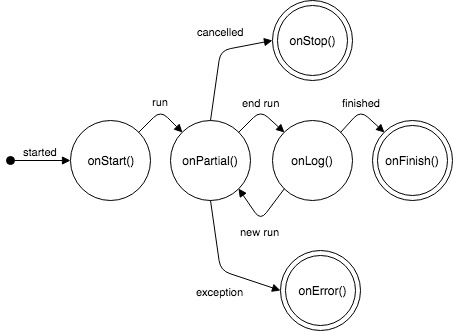
\includegraphics[width=\linewidth]{../figures/d14.jpg}
    \caption{Estados de un hilo de experiemento}
    \label{fig:d14}
\end{figure}

\newpage